\documentclass{beamer}
\usetheme[pageofpages=of,% String used between the current page and the
                         % total page count.
          bullet=circle,% Use circles instead of squares for bullets.
          titleline=true,% Show a line below the frame title.
          alternativetitlepage=true,% Use the fancy title page.
       %   titlepagelogo=logo-polito,% Logo for the first page.
       %   watermark=watermark-polito,% Watermark used in every page.
       %   watermarkheight=100px,% Height of the watermark.
       %   watermarkheightmult=4,% The watermark image is 4 times bigger
                                % than watermarkheight.
          ]{Torino}

\setbeamertemplate{footline}{
  \begin{beamercolorbox}[wd=\paperwidth,ht=1ex,dp=1ex]{footline}
    \vspace{5pt} \hspace{1em} \insertframenumber/\inserttotalframenumber
  \end{beamercolorbox}
}

\author{Brendon J. Brewer}
\title{STATS 331 -- Introduction to Bayesian Statistics}
\institute{The University of Auckland}
\date{}


\linespread{1.3}
\usepackage{minted}
\usepackage[utf8]{inputenc}
\usepackage{dsfont}


\begin{document}

\frame{\titlepage}

\begin{frame}
\frametitle{Welcome}
This lecture will just give an overview of the course.

\end{frame}


% New slide
\begin{frame}
\frametitle{Famous Bayesian Figures}

\begin{figure}[!h]
\centering
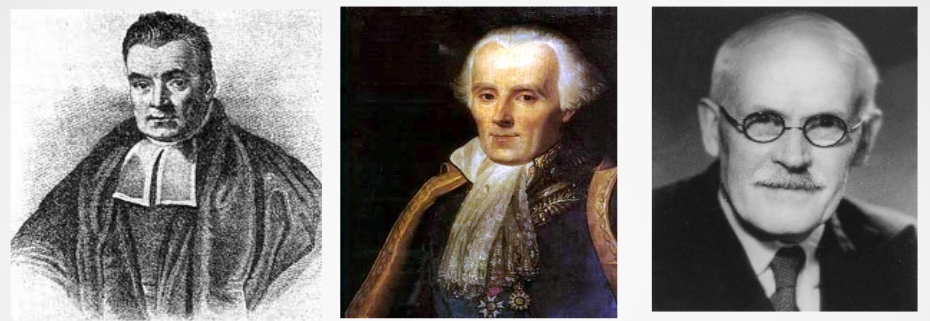
\includegraphics[width=0.8\textwidth]{images/people.png}
\caption{Thomas Bayes, Pierre-Simon Laplace, Harold Jeffreys
\label{fig:people}}
\end{figure}

\end{frame}


% New slide
\begin{frame}
\frametitle{Practicalities}
There are only two lectures per week, along with two lab sessions.
You should generally only come to one lab session, unless you want extra help. \\[1em]
\pause

All the course material will be available on Canvas.

\end{frame}


% New slide
\begin{frame}
\frametitle{Labs}

\begin{alertblock}{Lab Start Date}
There are no labs in Week 1. Labs will begin in Week 2.
\end{alertblock}\pause

\begin{alertblock}{Lab Attendance}
Lab attendance is not mandatory, but it will be much easier to
fully understand the material if you attend and attempt the questions.
\end{alertblock}

\end{frame}


% New slide
\begin{frame}
\frametitle{Grades and Assessment}
The grades available in this course are broken down as follows:\pause

\begin{itemize}
\item 24\% Assignments (Four assignments, each worth 6\%)\pause
\item 6\% Canvas quizzes (Two quizzes, each worth 3\%)\pause
\item 20\% Midterm Test (held in Week 7)\pause
\item 50\% Final Exam (two hours)\pause
\end{itemize}

\begin{alertblock}{Exam Minimum}
You must achieve 45\% on the final exam, as well as 50\% overall, to pass.
There is no plussage.
\end{alertblock}
\end{frame}


% New slide
\begin{frame}
\frametitle{The Four Assignments}
\begin{itemize}
\item The assignments will be uploaded to Canvas at least two weeks before they
are due.
\item The assignments are intended to be of medium difficulty and length.
\item Assignment submission will be via PDF upload on Canvas.
\end{itemize}

\end{frame}




% New slide
\begin{frame}
\frametitle{Class Representative}
We will need a class representative. Please see me at the end of this lecture
if you would like to volunteer. You will need to be available at the time of the
meetings.


\end{frame}


% New slide
\begin{frame}
\frametitle{Office Hours}
I will run one office hour each week, where you can ask me anything about the
course, including assignment help. The exact hour will be posted on Canvas. \pause

\begin{alertblock}{Office Location}
My office is room 331 (!) in Building 303 (the Science building).
\end{alertblock}
\end{frame}


% New slide
\begin{frame}
\frametitle{Lecture Notes and Books}
There are some PDF lecture notes (written a long time ago now, but with a
couple of recent updates) available on Canvas. These notes cover much of
the same material as lectures, but there are some topics that do not appear in
the notes.\\[1em] \pause

I will also suggest a couple of books which might be helpful.
\end{frame}


\begin{frame}
\frametitle{Books}
The book {\em Doing Bayesian Data Analysis: A Tutorial with R, JAGS, and Stan}
by John Krushcke covers roughly similar ground to STATS 331.
It is available online at the university library.
Plus it has dogs for some reason.

\begin{figure}[!h]
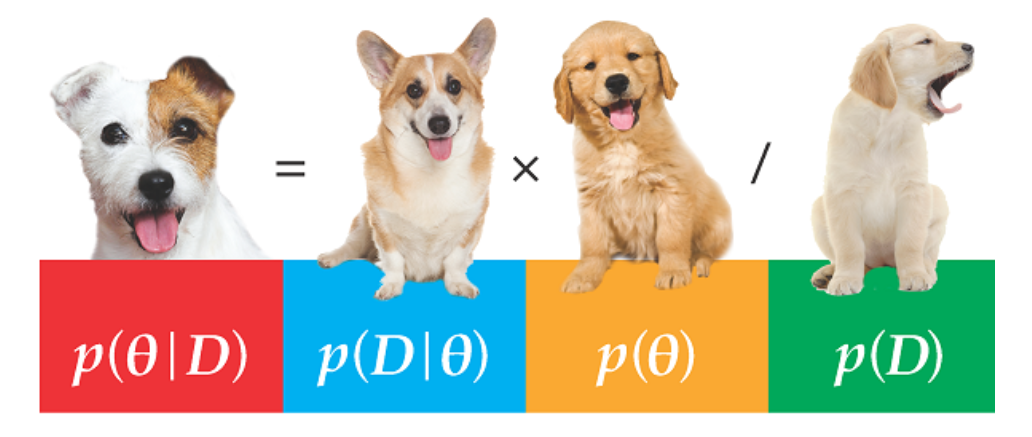
\includegraphics[width=0.7\textwidth]{images/dogs.png}
\caption{Dogs.\label{fig:dogs}}
\end{figure}

\end{frame}

\begin{frame}
\frametitle{Books}

    \begin{columns} % Create two columns
        \column{0.5\textwidth} % Left column (50% width)
        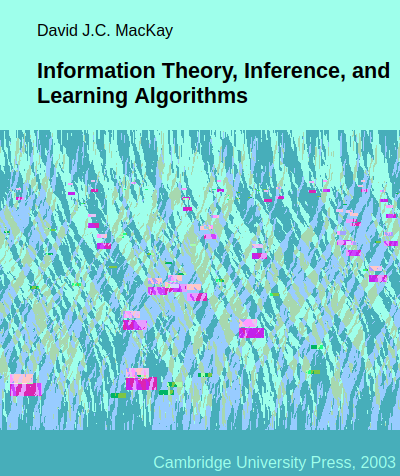
\includegraphics[width=0.8\linewidth]{images/itila.png}

        \column{0.5\textwidth} % Right column (50% width)
        \begin{itemize}
        \item This is an old book that covers Bayesian topics, but it also
        covers a lot more that is not relevant for STATS 331. I think it's an
        excellent book.\pause
        \item It is available online for free
            \href{http://www.inference.org.uk/itprnn/book.pdf}{here}, but you
            are not supposed to print it out.
        \end{itemize}
     \end{columns}

\end{frame}


\begin{frame}
\frametitle{Books}

    \begin{columns} % Create two columns
        \column{0.5\textwidth} % Left column (50% width)
        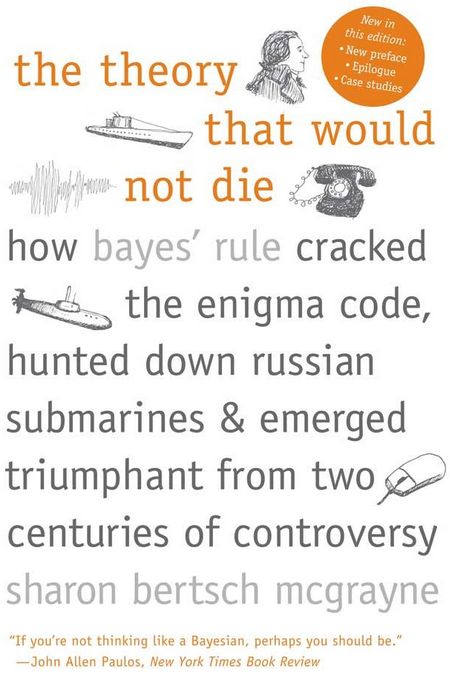
\includegraphics[width=0.7\linewidth]{images/theory.png}

        \column{0.5\textwidth} % Right column (50% width)
        \begin{itemize}
        \item This is a popular science book that you might enjoy.\pause
        \item There is an author talk about it which you can watch
            \href{https://www.youtube.com/watch?v=8oD6eBkjF9o}{here}.
        \end{itemize}
     \end{columns}

\end{frame}


\begin{frame}
\frametitle{Books}
These book suggestions are just that: suggestions. You are certaintly not
expected to read them, and I won't refer to them in class (although I do use
some MacKay questions in labs).

\end{frame}

\begin{frame}
\frametitle{Let's Get Started}

\begin{figure}[!h]
\centering
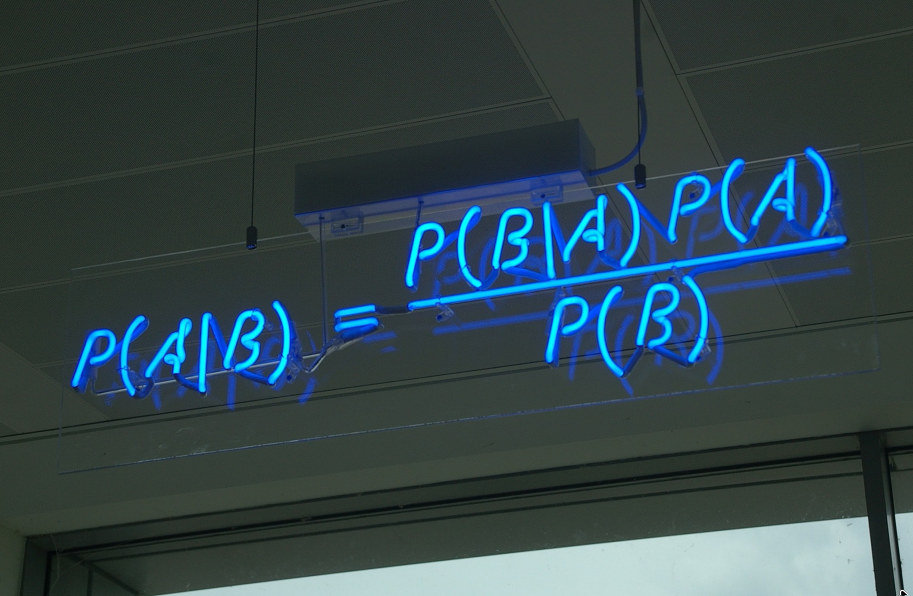
\includegraphics[width=0.8\textwidth]{images/neon.png}
\caption{Bayes' rule in neon. Credit: Matt Buck.}
\end{figure}

\end{frame}


\begin{frame}
\frametitle{Bayesian Statistics}
I am curious how many of you have heard of Bayesian statistics before
hearing about or enrolling in this course. Note that it sometimes goes by the
names {\em Bayesian Inference}, {\em Bayesian Analysis}, and
{\em probabilistic inference}.


\end{frame}

\begin{frame}
\frametitle{Bayesian Statistics}
The Bayesian approach is an alternative to methods such as
{\em p-values} and {\em confidence intervals} which you may have come across
in other courses.\pause

\begin{itemize}
\item It provides a clear, common-sense framework for
understanding and approaching statistics problems\pause
\item We will spend some time discussing the foundations of the
subject, and then we will see how to use it in common data analysis scenarios.
\end{itemize}


\end{frame}

\begin{frame}
\frametitle{Thomas Bayes (1701 -- 1761)}

    \begin{columns} % Create two columns
        \column{0.3\textwidth} % Left column (50% width)
        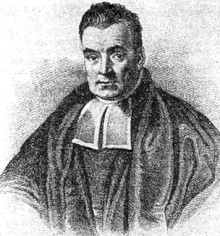
\includegraphics[width=1\linewidth]{images/bayes.jpg}

        \column{0.7\textwidth} % Right column (50% width)
        \begin{itemize}
        \item English clergyman/mathematician (possibly not really a picture of him)\pause
        \item Wrote a posthumously-published article that solved one particular problem in a ``Bayesian'' way
                (we will see what this means soon)
        \end{itemize}
     \end{columns}

\end{frame}


\begin{frame}
\frametitle{Pierre-Simon Laplace (1749 -- 1827)}

    \begin{columns} % Create two columns
        \column{0.3\textwidth} % Left column (50% width)
        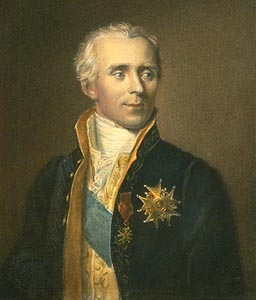
\includegraphics[width=1\linewidth]{images/laplace.jpg}

        \column{0.7\textwidth} % Right column (50% width)
        \begin{itemize}
        \item French mathematician/astronomer\pause
        \item Developed Bayes' ideas into a fully fledged theory and applied it
              to many scientific problems\pause
        \item He was unaware of Bayes' work at first,
              but acknowledged it later.\pause
        \item What we call `Bayes' rule' (we'll meet it soon)
              was first written down by Laplace.
        \end{itemize}
     \end{columns}

\end{frame}

\begin{frame}
\frametitle{Harold Jeffreys (1891 -- 1989)}

    \begin{columns} % Create two columns
        \column{0.3\textwidth} % Left column (50% width)
        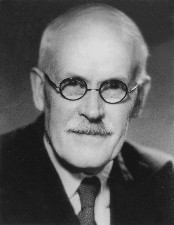
\includegraphics[width=1\linewidth]{images/jeffreys.jpg}

        \column{0.7\textwidth} % Right column (50% width)
        \begin{itemize}
        \item English geophysicist active in the 20th century\pause
        \item When Bayesian ideas were under attack [and ``statistics'' was
              on the rise due to Ronald Fisher and others], he defended them
              and developed them further\pause
        \item Wrote an important textbook, {\em Theory of Probability}.
        \end{itemize}
     \end{columns}

\end{frame}


\end{document}

